%% !TEX program = pdflatex
%% !BIB program = bibtex
\documentclass[12pt]{article}

\usepackage{amsfonts,amsmath,amssymb,mathtools,marvosym}
\usepackage[left=2.5cm,right=2cm,top=2cm,bottom=2.5cm]{geometry}
\usepackage{indentfirst,setspace,multirow}
\usepackage{graphicx,xcolor,float,epstopdf}
\usepackage{enumerate}
\usepackage[bookmarks=true,breaklinks=true,colorlinks,linkcolor=blue,citecolor=blue,urlcolor=blue]{hyperref}

\usepackage{array}
\newcolumntype{P}[1]{>{\centering\arraybackslash}p{#1}}
\newcolumntype{M}[1]{>{\centering\arraybackslash}m{#1}}
\newcolumntype{N}[1]{>{\arraybackslash}m{#1}}

\onehalfspacing
%\doublespacing

\setlength{\parindent}{0.5cm}
\setlength{\parskip}{0cm}
%\renewcommand{\baselinestretch}{1.15} % 1.6 for double

% ==============================================================================

\title{\textbf{Quiz 1}}
\author{ECON312 Time Series Analysis \\ Instructor: Narek Ohanyan}
\date{}

\begin{document}

\maketitle

\vspace{1cm}

\textbf{Student} $ \qquad \underset{\text{first name}}{\underline{\hspace{4cm}}} \quad \underset{\text{last name}}{\underline{\hspace{6cm}}}  $

\bigskip
\textbf{Grade} $ \qquad \underline{\hspace{1cm}} \quad / \quad 10 $

% ------------------------------------------------------------------------------

\vspace{1cm}

\section*{Instructions}

\begin{itemize}
    \item The quiz is closed-book.
    \item No electronic devices are allowed.
    \item Write your answers in a clear and unambiguous way.

          Good luck!
\end{itemize}

% ==============================================================================

\newpage

\section*{Question 1 \normalfont{\normalsize{(2 pts.)}}}

Suppose the you have time series data on some variable $ y_{t} $, and you want to determine whether the series is $ AR(p) $ or $ MA(q) $ along with the order of the process $ p $ or $ q $.

The figures below show the ACF and PACF of the series. Based on the information provided in the figure determine the type of the process, i.e. $ AR $ or $ MA $, and the order of the process $ p $ or $ q $.

\begin{figure}[H]
    \centering
    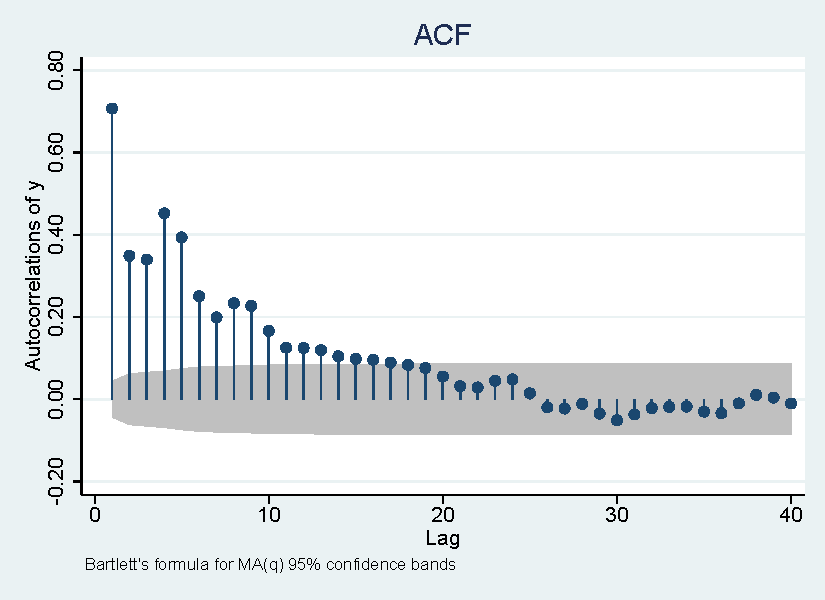
\includegraphics[width=0.45\textwidth]{./stata/fig/acf.pdf}
    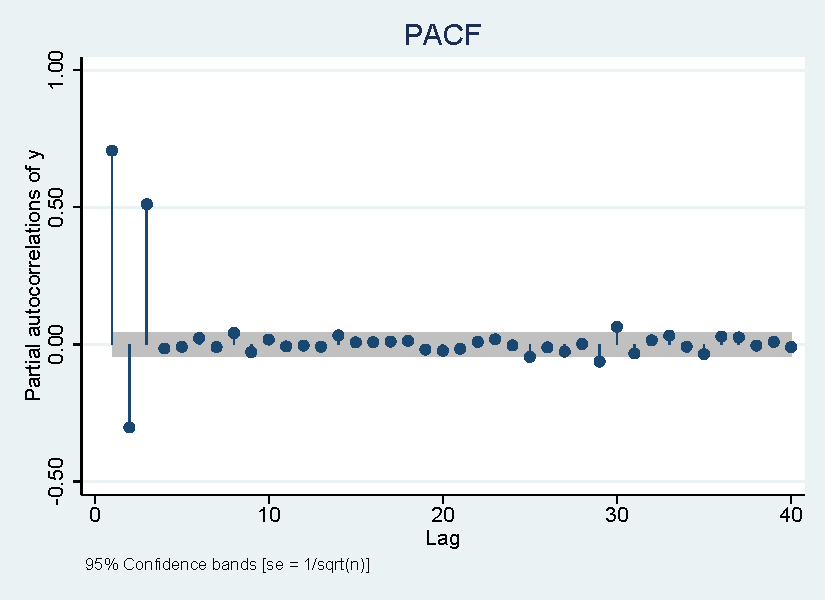
\includegraphics[width=0.45\textwidth]{./stata/fig/pacf.pdf}
\end{figure}

Explain your answer.

\vspace{5cm}

\section*{Question 2 \normalfont{\normalsize{(4 pts.)}}}

Consider the following $ AR(1) $ process:
\begin{equation*}
    y_{t} = \phi y_{t-1} + e_{t} \qquad e_{t} \sim WN(0, \sigma^{2})
\end{equation*}
with $ \phi = 0.6 $ and $ \sigma^{2} = 1 $.

Evaluate the following expressions:
\begin{itemize}
    \item $ \mathrm{Cov} \left( e_{t}, e_{t-1} \right) = $
          \vspace{2cm}
    \item $ \mathrm{Cov} \left( e_{t}, y_{t-1} \right) = $
          \vspace{2cm}
    \item $ \mathrm{Corr} \left( y_{t}, y_{t-1} \right) = $
          \vspace{2cm}
    \item $ \mathrm{Corr} \left( y_{t}, y_{t-2} \right) = $
          \vspace{2cm}
\end{itemize}

% ------------------------------------------------------------------------------

\section*{Question 3 \normalfont{\normalsize{(4 pts.)}}}

Consider the following process:
\begin{equation*}
    y_{t} = c + e_{t} + \theta_1 e_{t-1} + \theta_2 e_{t-2} \qquad e_{t} \sim WN(0, \sigma^{2})
\end{equation*}

Evaluate the following expressions:
\begin{itemize}
    \item $ \mathrm{Var} \left( y_{t} \right) = $
          \vspace{2cm}
    \item $ \mathrm{Cov} \left( y_{t}, y_{t-1} \right) = $
          \vspace{2cm}
    \item $ \mathrm{Cov} \left( y_{t}, e_{t-2} \right) = $
          \vspace{2cm}
    \item $ \mathrm{Cov} \left( y_{t}, e_{t-3} \right) = $
          \vspace{2cm}
\end{itemize}

% ==============================================================================

\end{document}